% Name: Feedback control loop
% Description: A controller and a plant with the output measured and fed back to a summing junction.
% Tags: feedback, control loop, transfer function

\usetikzlibrary{arrows.meta, positioning}

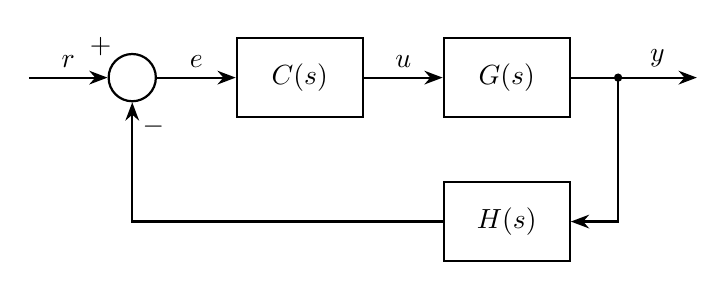
\begin{tikzpicture}[
  node distance=8mm and 10mm,
  block/.style={draw, thick, minimum height=10mm, minimum width=16mm},
  sum/.style={draw, thick, circle, inner sep=0pt, minimum size=6mm},
  arrow/.style={-{Stealth}, thick},
]
  \coordinate (in);
  \node[sum, right=of in] (sum) {};
  \node[block, right=of sum] (ctrl) {$C(s)$};
  \node[block, right=of ctrl] (plant) {$G(s)$};
  \coordinate[right=6mm of plant] (tap);
  \coordinate[right=10mm of tap] (out);
  \node[block, below=of plant] (sensor) {$H(s)$};

  \draw[arrow] (in) -- node[above] {$r$} (sum);
  \draw[arrow] (sum) -- node[above] {$e$} (ctrl);
  \draw[arrow] (ctrl) -- node[above] {$u$} (plant);
  \draw[thick] (plant) -- (tap);
  \draw[arrow] (tap) -- node[above] {$y$} (out);
  \draw[arrow] (tap) |- (sensor);
  \draw[arrow] (sensor) -| node[pos=0.9, right] {$-$} (sum);
  \fill (tap) circle (1.5pt);
  \node at ([shift={(-4mm,4mm)}]sum) {$+$};
\end{tikzpicture}
